\begin{figure*}
    \centering
    \begin{subfigure}[b]{0.32\textwidth}
        \centering
        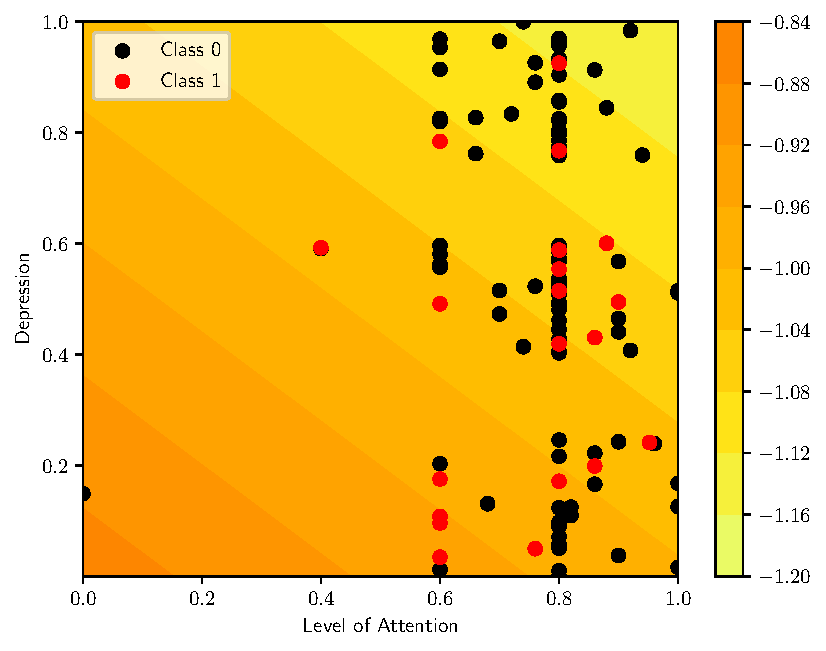
\includegraphics[width=\textwidth]{figs/svm-linear-contour-0-3.pdf}
        \caption{}
    \end{subfigure}
    \begin{subfigure}[b]{0.32\textwidth}
        \centering
        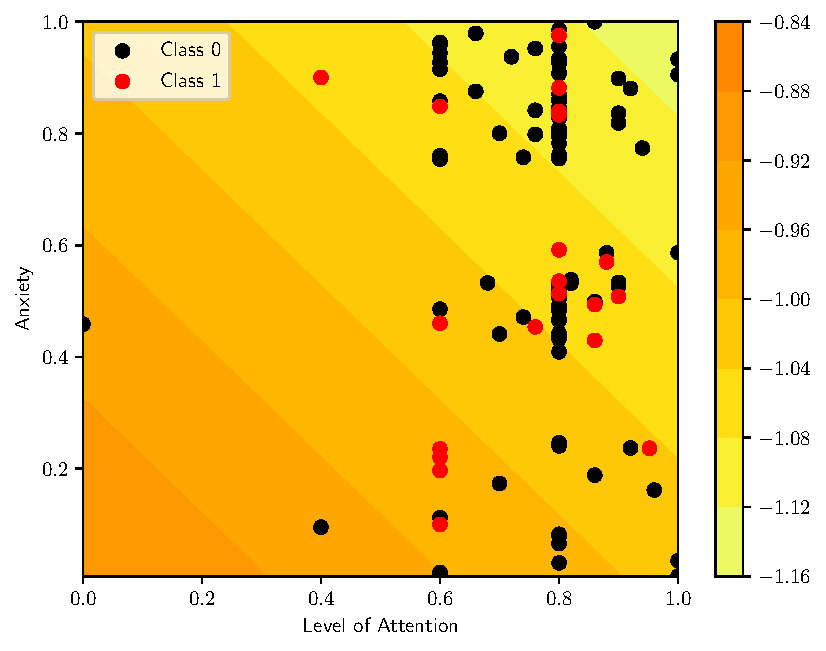
\includegraphics[width=\textwidth]{figs/svm-linear-contour-0-4.pdf}
        \caption{}
    \end{subfigure}
    \begin{subfigure}[b]{0.32\textwidth}
        \centering
        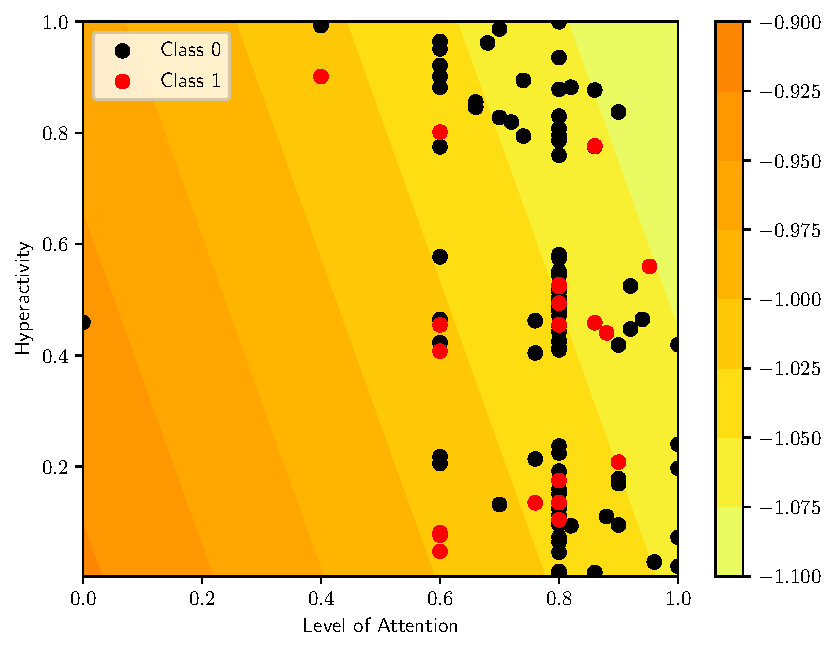
\includegraphics[width=\textwidth]{figs/svm-linear-contour-0-5.pdf}
        \caption{}
    \end{subfigure}

    \begin{subfigure}[b]{0.32\textwidth}
        \centering
        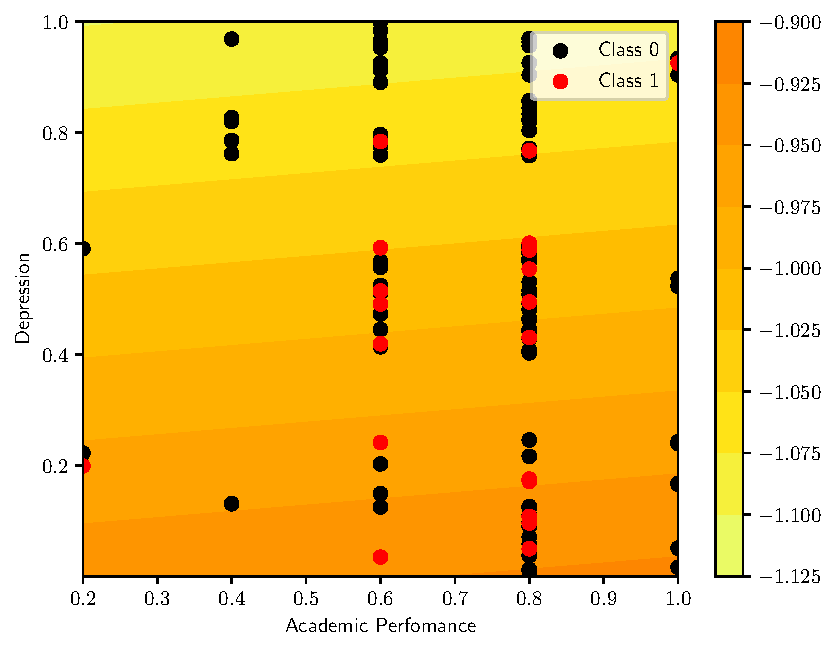
\includegraphics[width=\textwidth]{figs/svm-linear-contour-1-3.pdf}
        \caption{}
    \end{subfigure}
    \begin{subfigure}[b]{0.32\textwidth}
        \centering
        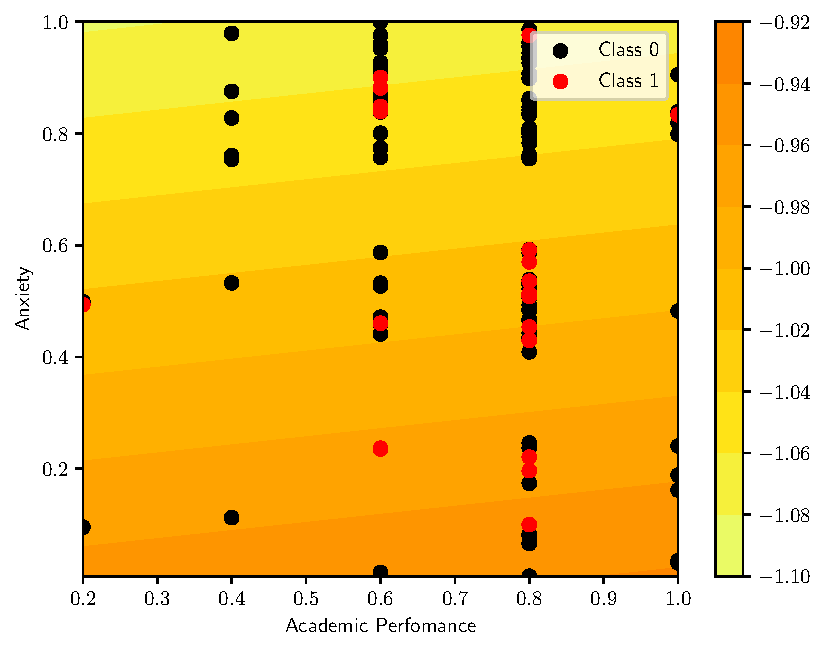
\includegraphics[width=\textwidth]{figs/svm-linear-contour-1-4.pdf}
        \caption{}
    \end{subfigure}
    \begin{subfigure}[b]{0.32\textwidth}
        \centering
        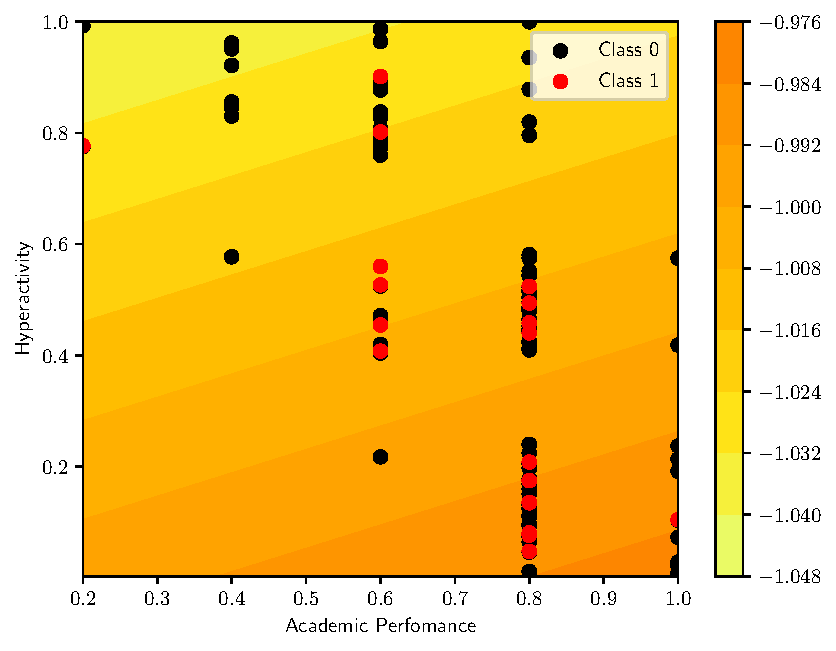
\includegraphics[width=\textwidth]{figs/svm-linear-contour-1-5.pdf}
        \caption{}
    \end{subfigure}

    \begin{subfigure}[b]{0.32\textwidth}
        \centering
        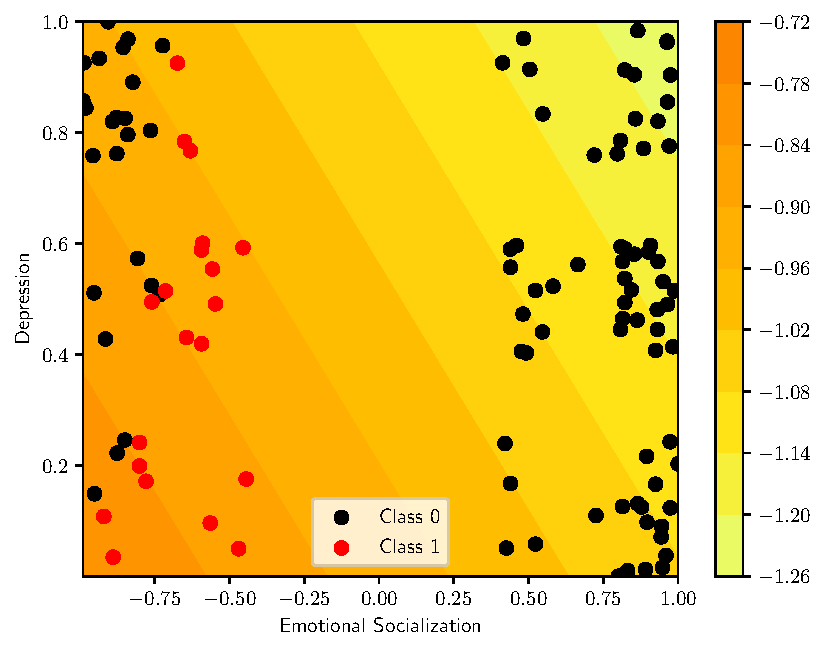
\includegraphics[width=\textwidth]{figs/svm-linear-contour-2-3.pdf}
        \caption{}
    \end{subfigure}
    \begin{subfigure}[b]{0.32\textwidth}
        \centering
        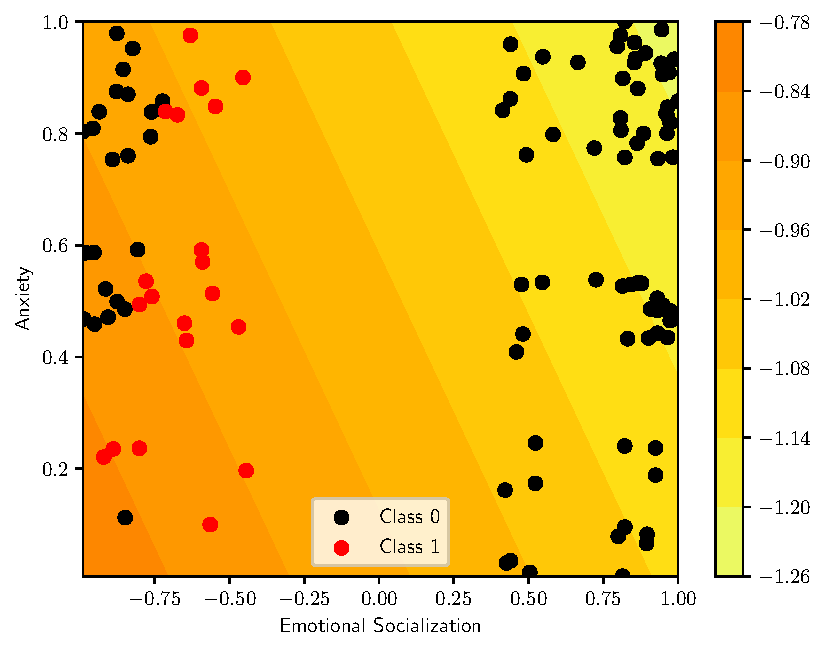
\includegraphics[width=\textwidth]{figs/svm-linear-contour-2-4.pdf}
        \caption{}
    \end{subfigure}
    \begin{subfigure}[b]{0.32\textwidth}
        \centering
        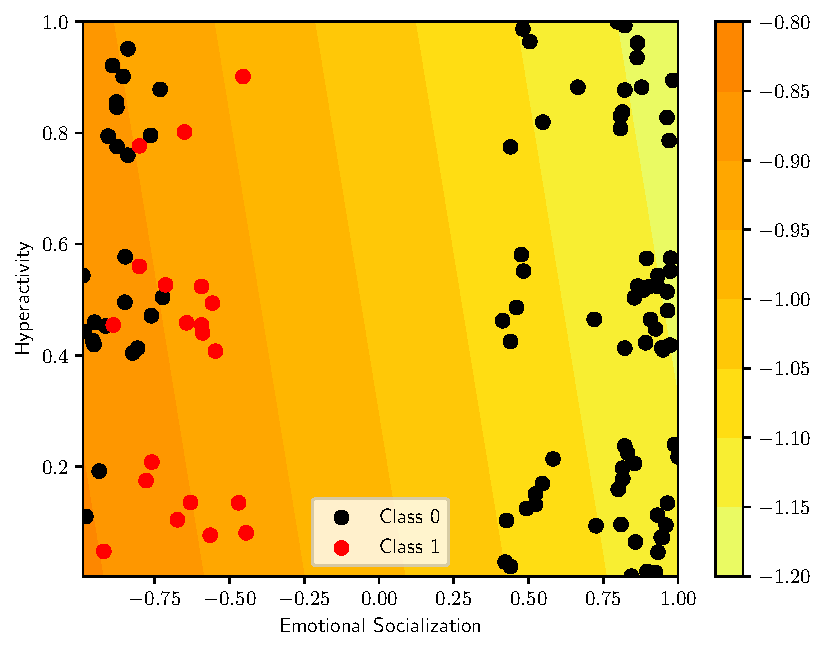
\includegraphics[width=\textwidth]{figs/svm-linear-contour-2-5.pdf}
        \caption{}
    \end{subfigure}
    \caption{Linear kernel SVM contour with real labels.}
    \label{fig:SVM-linear}
\end{figure*}

\begin{figure*}
    \centering
    \begin{subfigure}[b]{0.32\textwidth}
        \centering
        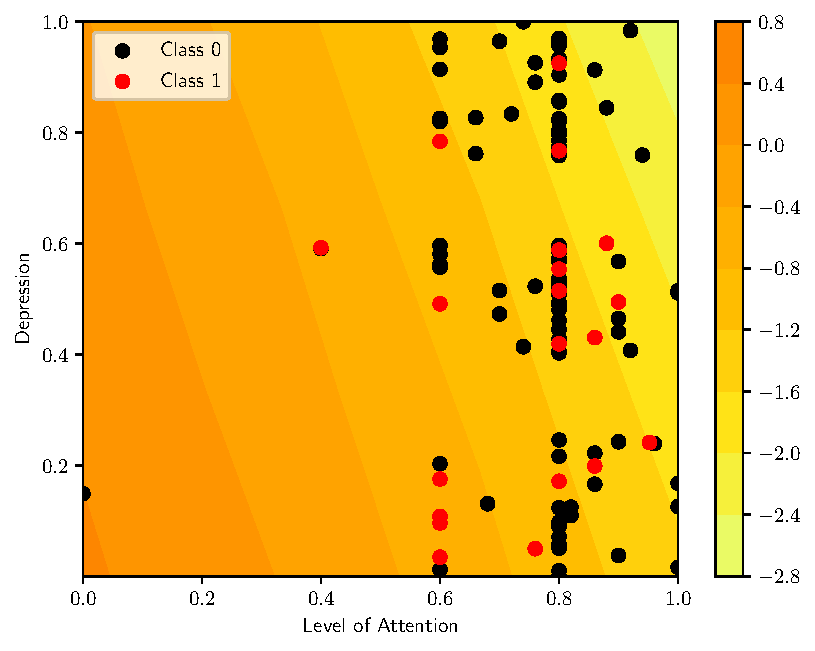
\includegraphics[width=\textwidth]{figs/svm-poly-contour-0-3.pdf}
        \caption{}
    \end{subfigure}
    \begin{subfigure}[b]{0.32\textwidth}
        \centering
        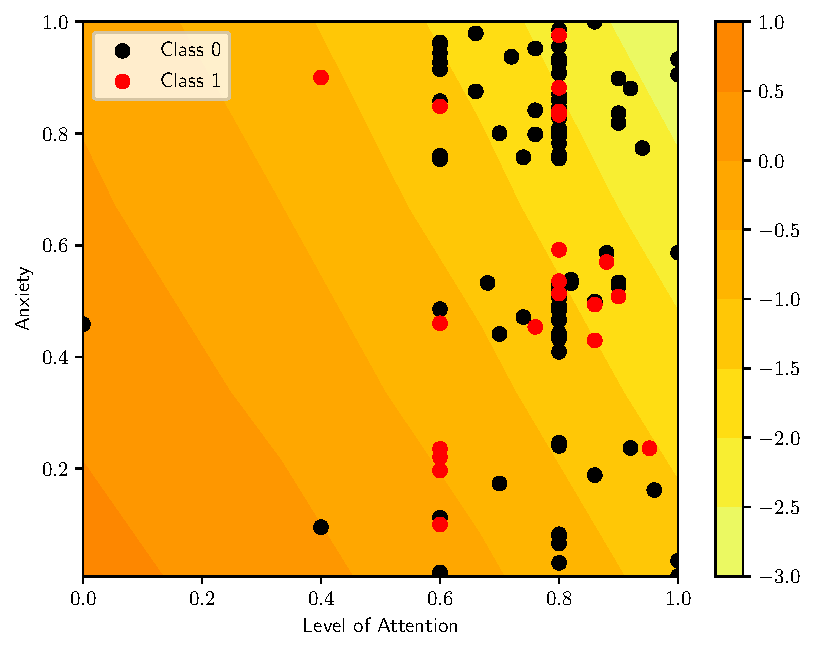
\includegraphics[width=\textwidth]{figs/svm-poly-contour-0-4.pdf}
        \caption{}
    \end{subfigure}
    \begin{subfigure}[b]{0.32\textwidth}
        \centering
        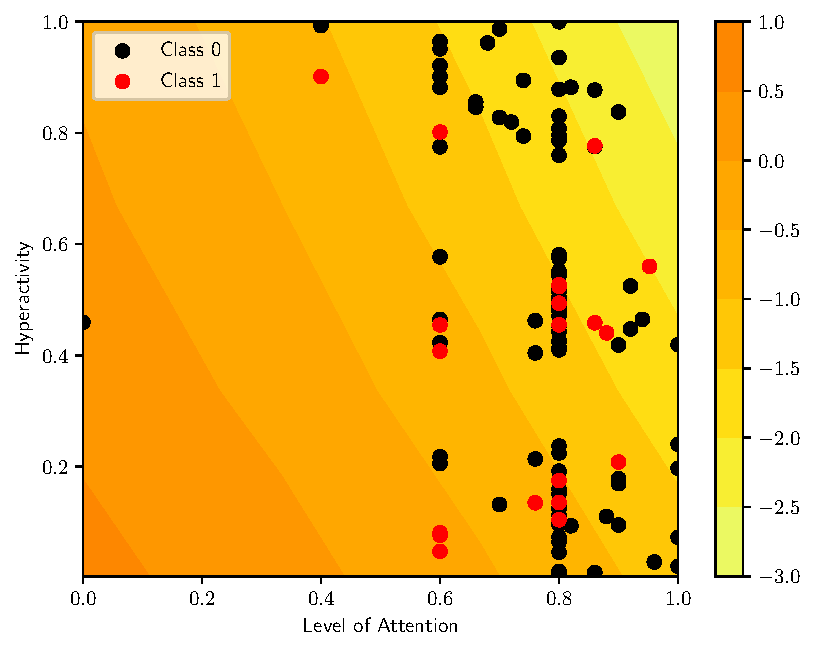
\includegraphics[width=\textwidth]{figs/svm-poly-contour-0-5.pdf}
        \caption{}
    \end{subfigure}

    \begin{subfigure}[b]{0.32\textwidth}
        \centering
        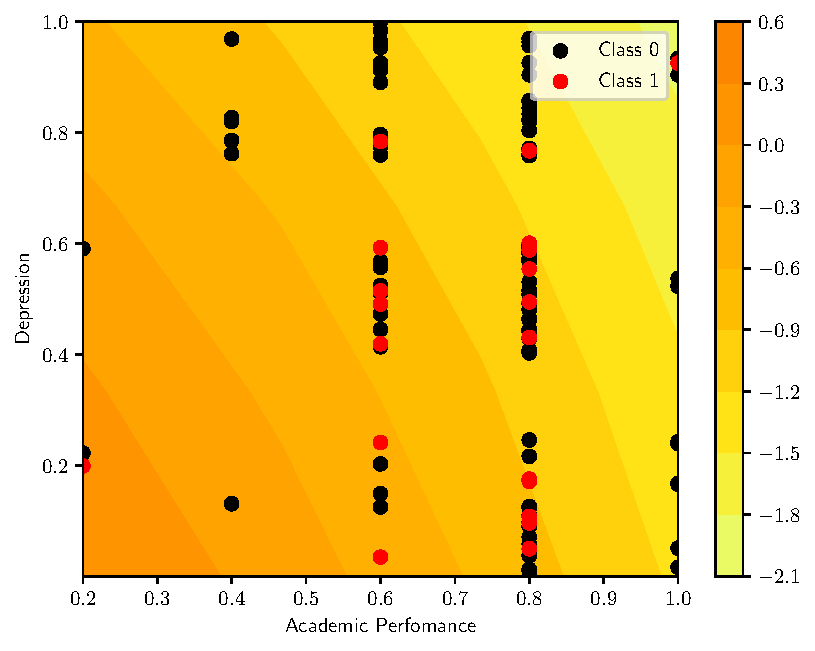
\includegraphics[width=\textwidth]{figs/svm-poly-contour-1-3.pdf}
        \caption{}
    \end{subfigure}
    \begin{subfigure}[b]{0.32\textwidth}
        \centering
        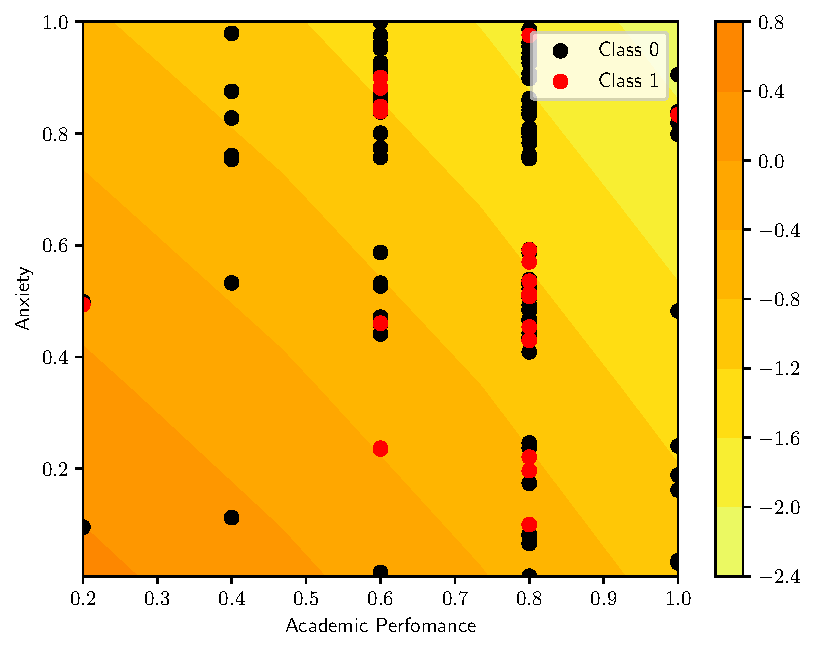
\includegraphics[width=\textwidth]{figs/svm-poly-contour-1-4.pdf}
        \caption{}
    \end{subfigure}
    \begin{subfigure}[b]{0.32\textwidth}
        \centering
        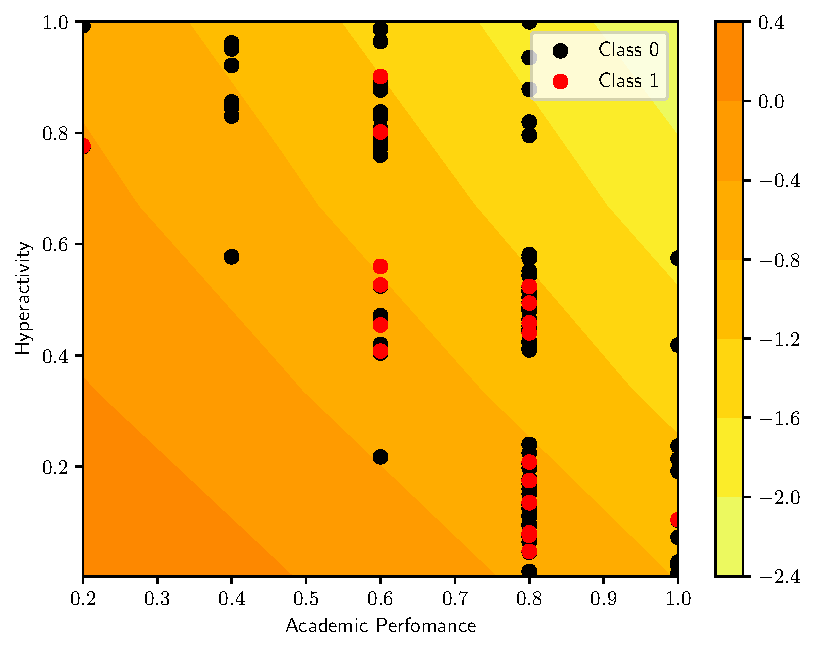
\includegraphics[width=\textwidth]{figs/svm-poly-contour-1-5.pdf}
        \caption{}
    \end{subfigure}

    \begin{subfigure}[b]{0.32\textwidth}
        \centering
        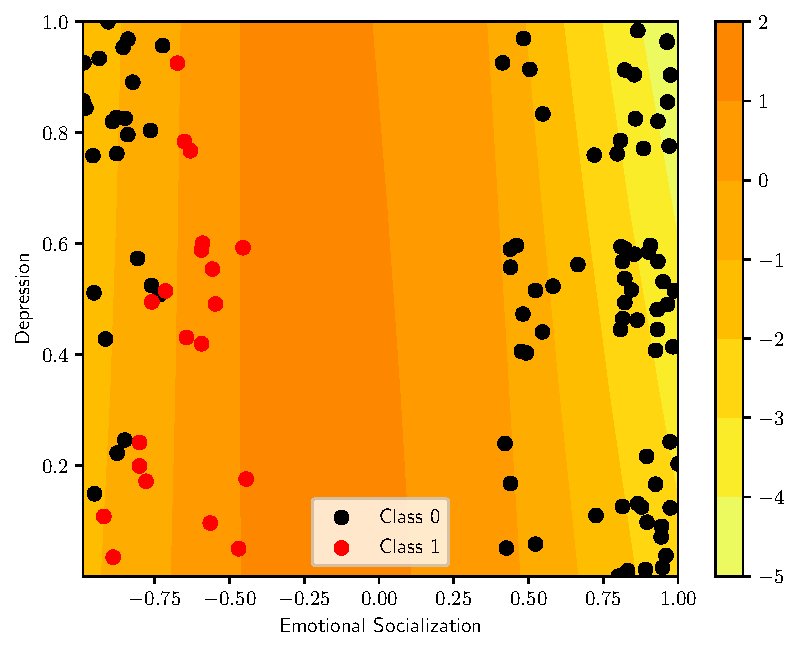
\includegraphics[width=\textwidth]{figs/svm-poly-contour-2-3.pdf}
        \caption{}
    \end{subfigure}
    \begin{subfigure}[b]{0.32\textwidth}
        \centering
        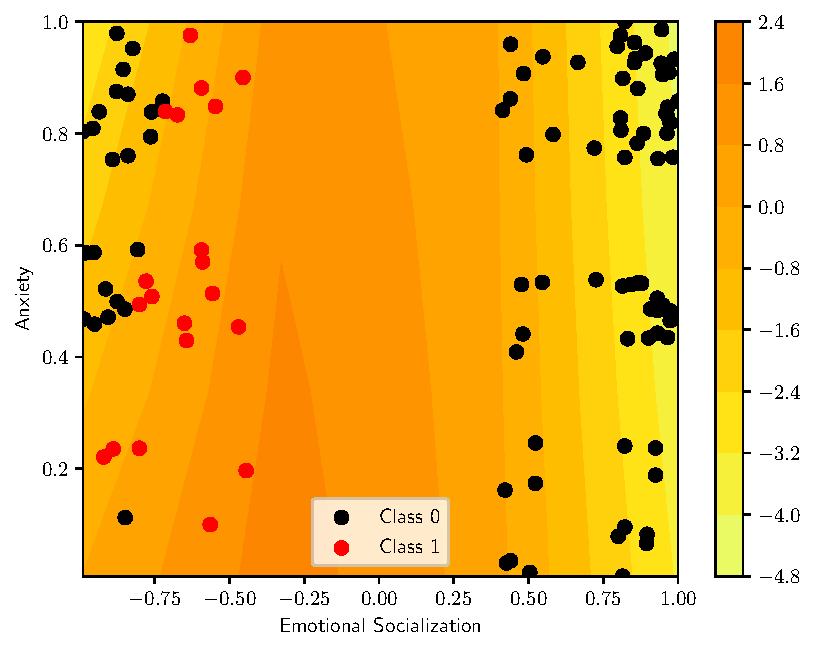
\includegraphics[width=\textwidth]{figs/svm-poly-contour-2-4.pdf}
        \caption{}
    \end{subfigure}
    \begin{subfigure}[b]{0.32\textwidth}
        \centering
        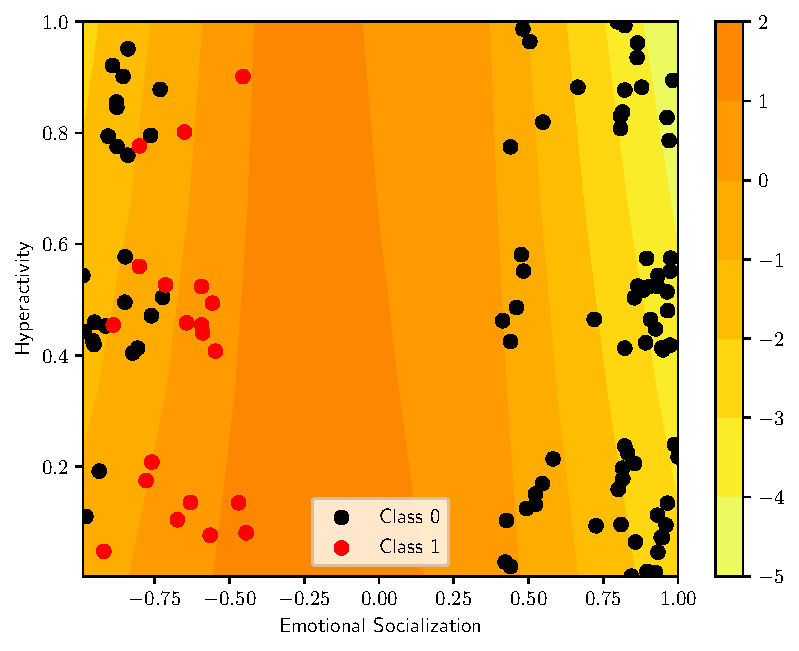
\includegraphics[width=\textwidth]{figs/svm-poly-contour-2-5.pdf}
        \caption{}
    \end{subfigure}
    \caption{Polynomial kernel SVM contour with real labels.}
    \label{fig:SVM-poly}
\end{figure*}

\begin{figure*}
    \centering
    \begin{subfigure}[b]{0.32\textwidth}
        \centering
        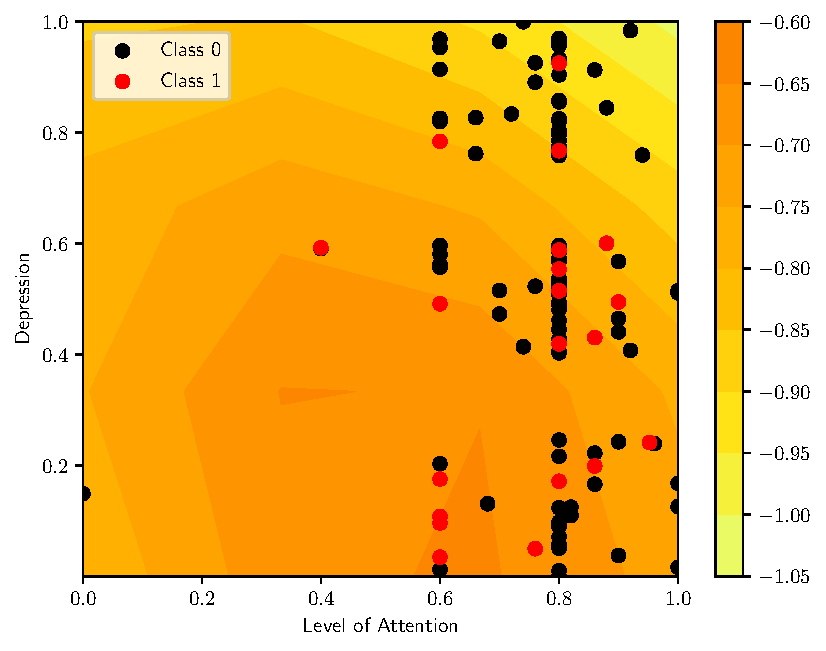
\includegraphics[width=\textwidth]{figs/svm-rbf-contour-0-3.pdf}
        \caption{}
    \end{subfigure}
    \begin{subfigure}[b]{0.32\textwidth}
        \centering
        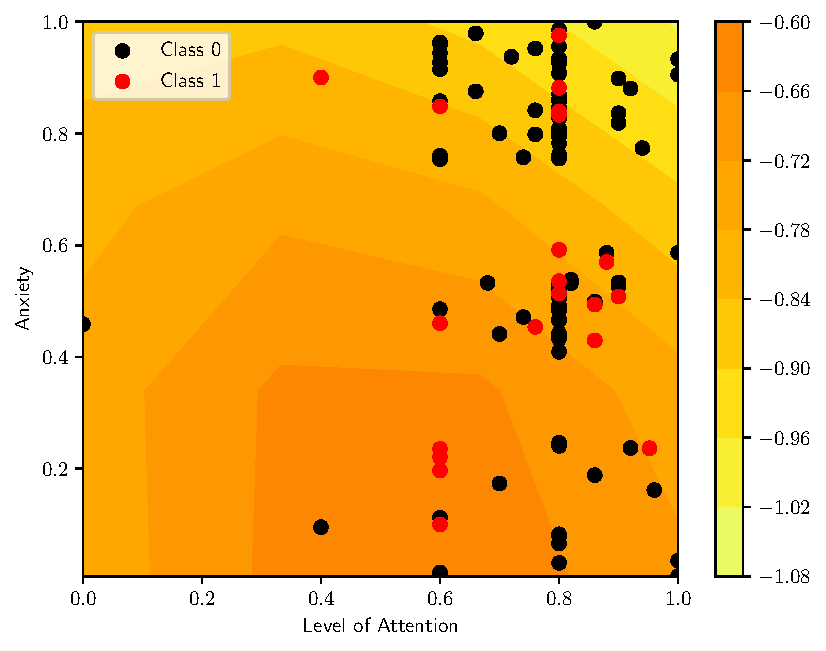
\includegraphics[width=\textwidth]{figs/svm-rbf-contour-0-4.pdf}
        \caption{}
    \end{subfigure}
    \begin{subfigure}[b]{0.32\textwidth}
        \centering
        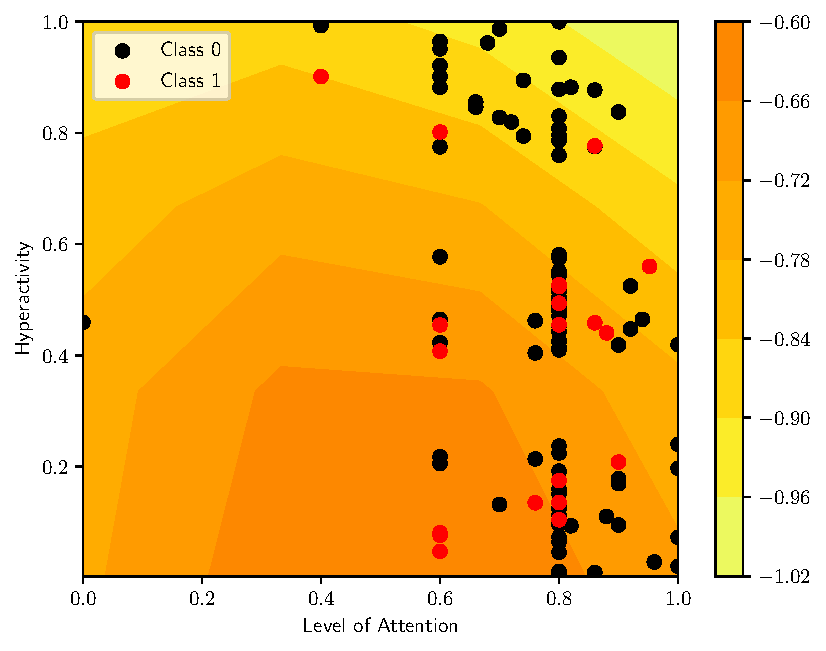
\includegraphics[width=\textwidth]{figs/svm-rbf-contour-0-5.pdf}
        \caption{}
    \end{subfigure}

    \begin{subfigure}[b]{0.32\textwidth}
        \centering
        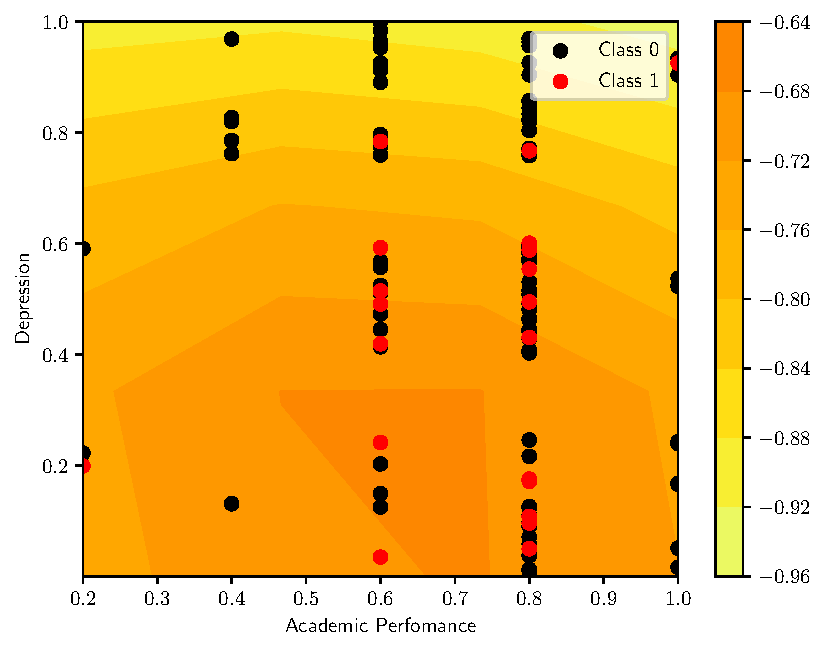
\includegraphics[width=\textwidth]{figs/svm-rbf-contour-1-3.pdf}
        \caption{}
    \end{subfigure}
    \begin{subfigure}[b]{0.32\textwidth}
        \centering
        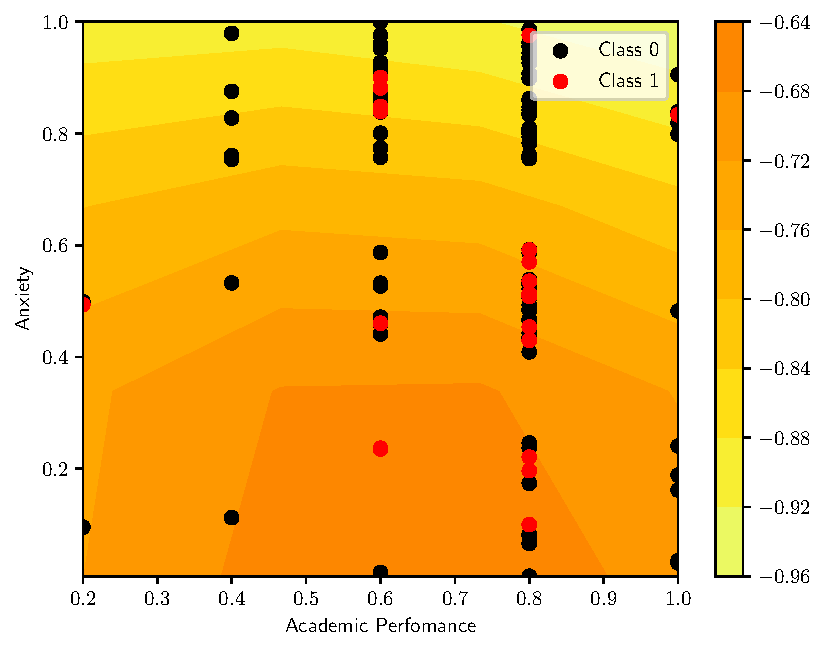
\includegraphics[width=\textwidth]{figs/svm-rbf-contour-1-4.pdf}
        \caption{}
    \end{subfigure}
    \begin{subfigure}[b]{0.32\textwidth}
        \centering
        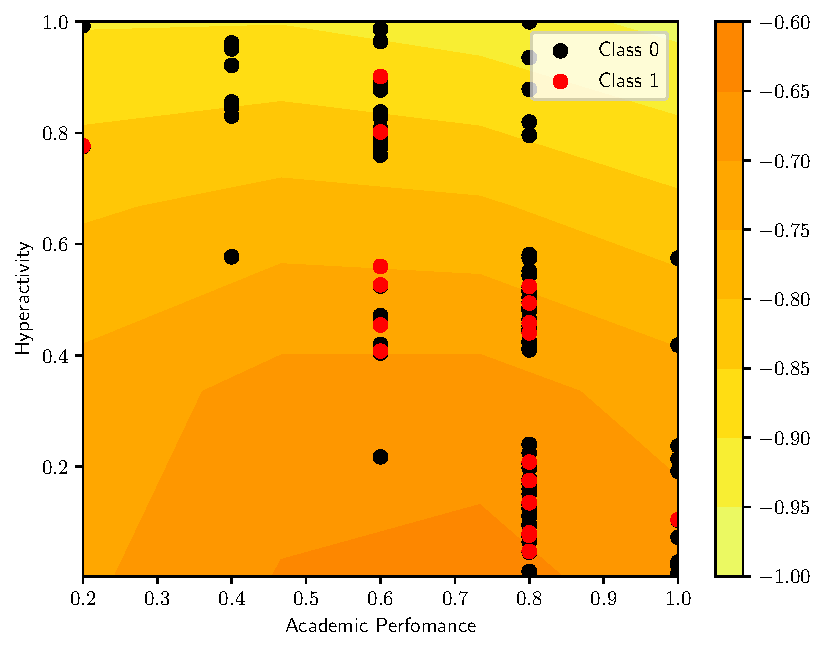
\includegraphics[width=\textwidth]{figs/svm-rbf-contour-1-5.pdf}
        \caption{}
    \end{subfigure}

    \begin{subfigure}[b]{0.32\textwidth}
        \centering
        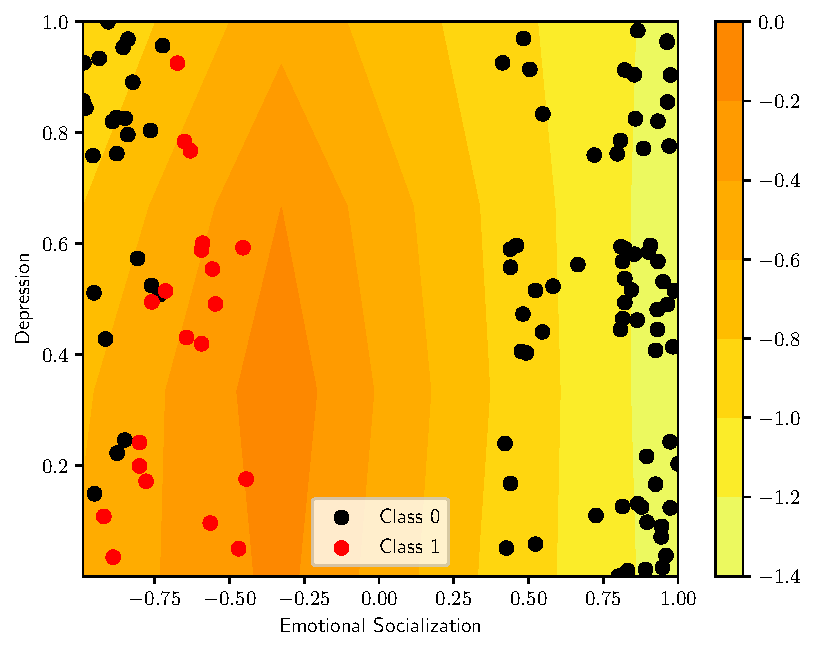
\includegraphics[width=\textwidth]{figs/svm-rbf-contour-2-3.pdf}
        \caption{}
    \end{subfigure}
    \begin{subfigure}[b]{0.32\textwidth}
        \centering
        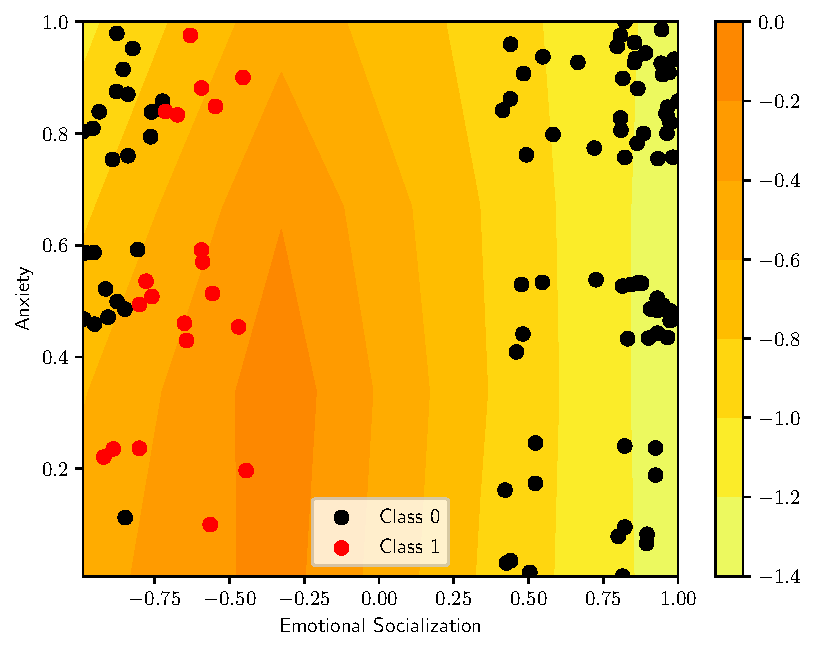
\includegraphics[width=\textwidth]{figs/svm-rbf-contour-2-4.pdf}
        \caption{}
    \end{subfigure}
    \begin{subfigure}[b]{0.32\textwidth}
        \centering
        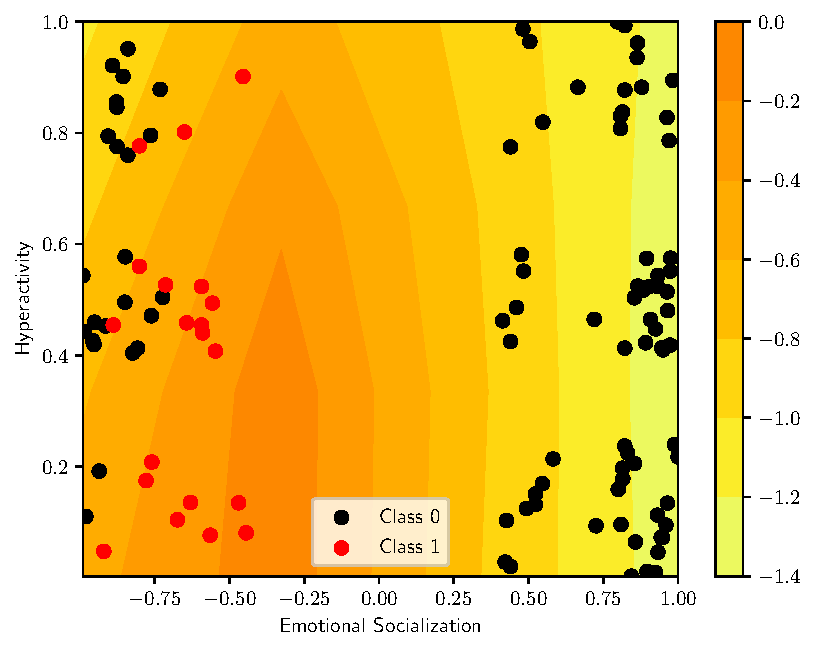
\includegraphics[width=\textwidth]{figs/svm-rbf-contour-2-5.pdf}
        \caption{}
    \end{subfigure}
    \caption{RBF kernel SVM contour with real labels.}
    \label{fig:SVM-rbf}
\end{figure*}

\begin{table}
\centering
\caption{Performance scores for linear SVM.}
\label{tab:linear_SVM}
\begin{tabular}{ccc}
\hline
\textbf{Set} & \textbf{Sensitivity} & \textbf{Specificity} \\ \hline
Training & 0 & 1 \\
Testing & 0 & 1 \\
Validation & 0 & 1 \\ \hline
\end{tabular}
\end{table}

\begin{table}
\centering
\caption{Performance scores for polynomial SVM.}
\label{tab:poly_SVM}
\begin{tabular}{cll}
\hline
\textbf{Set} & \multicolumn{1}{c}{\textbf{Sensitivity}} & \multicolumn{1}{c}{\textbf{Specificity}} \\ \hline
Training & 0.89 & 1 \\
Testing & 0 & 1 \\
Validation & 0.57 & 1 \\ \hline
\end{tabular}
\end{table}

\begin{table}
\centering
\caption{Performance scores for RBF SVM.}
\label{tab:rbf_SVM}
\begin{tabular}{cll}
\hline
\textbf{Set} & \multicolumn{1}{c}{\textbf{Sensitivity}} & \multicolumn{1}{c}{\textbf{Specificity}} \\ \hline
Training & 0.13 & 1 \\
Testing & 0 & 1 \\
Validation & 0.25 & 1 \\ \hline
\end{tabular}
\end{table}
